נתונים $n$ אינטרוולים
$A = \{a_1, \ldots, a_n\}$, 
נסמן ב-%
$s(a_i)$
את זמן ההתחלה של האינטרוול 
$a_i$
וב-%
$e(a_i)$
את זמן הסיום שלו.
לכל אינטרוול מתקיים ש-%
$s(a_i), e(a_i) \in \mathbb{R}_+$
וכן 
$s(a_i) < e(a_i)$
רוצים למצוא תת קבוצה בגודל מקסימלי
$I \subseteq A$
כך שהאינטרוולים ב-$I$ זרים בזוגות, כלומר לכל 
$a,b \in I$, 
אחד התנאים מתקיים:
$e(a) < s(b)$
או ש-%
$e(b) < s(a)$.

דוגמה:

\begin{center}
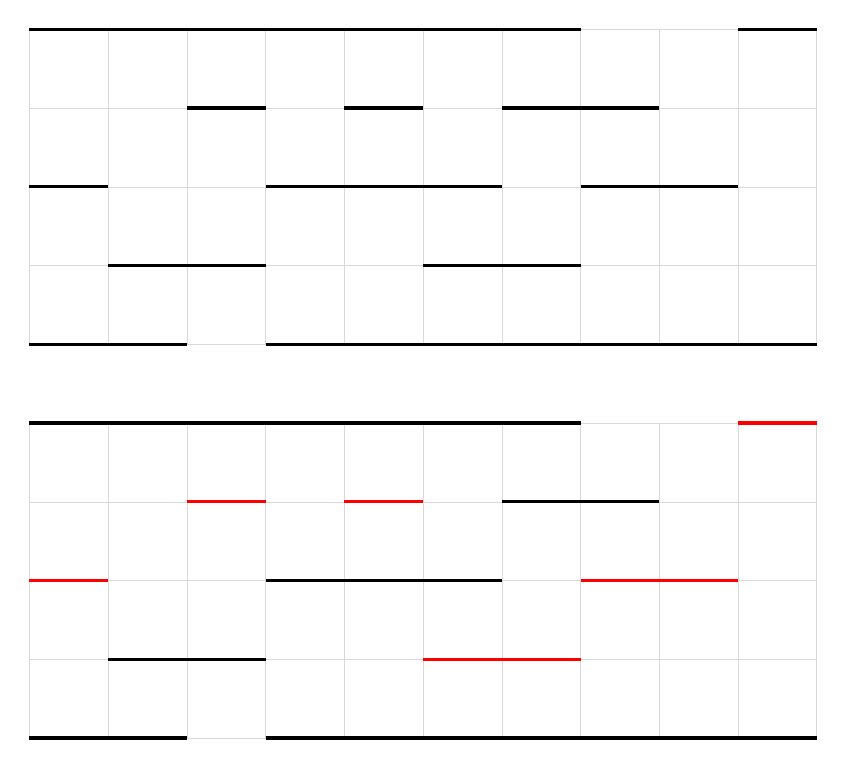
\begin{tikzpicture}[very thick]
\draw[very thin, gray!30] (0,0) grid (10, 4);
\draw (0,0) -- (2,0);
\draw (3,0) -- (10,0);

\draw (1,1) -- (3,1);
\draw (5,1) -- (7,1);

\draw (0,2) -- (1,2);
\draw (3,2) -- (6,2);
\draw (7,2) -- (9,2);

\draw (2,3) -- (3,3);
\draw (4,3) -- (5,3);
\draw (6,3) -- (8,3);

\draw (0,4) -- (7,4);
\draw (9,4) -- (10,4);

\begin{scope}[yshift=-5cm]
\draw[very thin, gray!30] (0,0) grid (10, 4);
\draw (0,0) -- (2,0);
\draw (3,0) -- (10,0);

\draw (1,1) -- (3,1);
\draw[red] (5,1) -- (7,1);

\draw[red] (0,2) -- (1,2);
\draw (3,2) -- (6,2);
\draw[red] (7,2) -- (9,2);

\draw[red] (2,3) -- (3,3);
\draw[red] (4,3) -- (5,3);
\draw (6,3) -- (8,3);

\draw (0,4) -- (7,4);
\draw[red] (9,4) -- (10,4);
\end{scope}

\end{tikzpicture}
\end{center}

אלגוריתם חמדן:
\begin{enumerate}
\item
אתחול:
$I \leftarrow \emptyset$, 
$\bar{e} \leftarrow 0$
\item
עבור כל אינטרוול 
$a$
בסדר לא יורד של ערכי 
$e(a)$:
	\begin{enumerate}
	\item
	אם 
	$s(a) \geq \bar{e}$
		\begin{enumerate}
		\item
		$I \leftarrow I \cup \{a\}$
		\item
		$\bar{e} \leftarrow e(a)$
		\end{enumerate}

	\end{enumerate}
\end{enumerate}
לפני שנוכיח נכונות נראה דוגמאות לגישות חמדניות שלא עובדות:

לבחור את האינטרוול עם זמן התחלה הכי מוקדם
\begin{center}
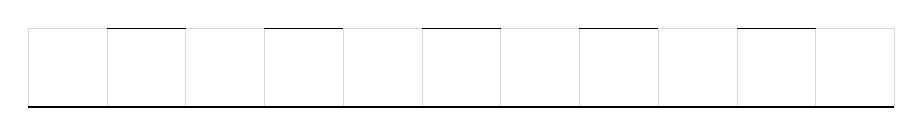
\begin{tikzpicture}
\draw[very thin, gray!30] (0,0) grid (11,1);
\draw (0,0) -- (11,0);
\foreach \s in {1,3,...,9}{
    \pgfmathsetmacro\e{\s + 1}
    \draw (\s, 1) -- (\e, 1);
}
\end{tikzpicture}
\end{center}

לבחור את האינטרוול הכי קצר
\begin{center}
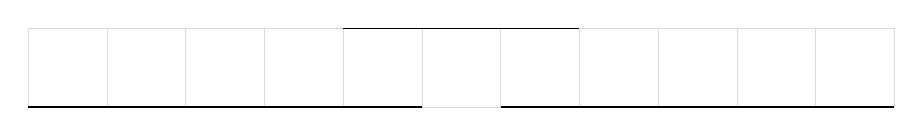
\begin{tikzpicture}
\draw[very thin, gray!30] (0,0) grid (11,1);
\draw (0,0) -- (5,0);
\draw (6,0) -- (11,0);
\draw (4,1) -- (7,1);
\end{tikzpicture}
\end{center}

לבחור את האינטרוול שנחתך עם הכי מעט אינטרוולים
\begin{center}
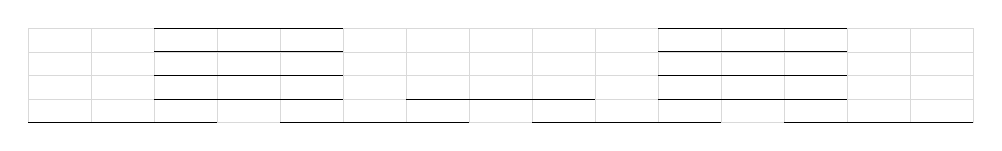
\begin{tikzpicture}[y=3mm, x=8mm]
\draw[very thin, gray!30, ystep=3mm, xstep=8mm] (0,0) grid (15,4);
\draw (0,0) -- (3,0);
\draw (4,0) -- (7,0);
\draw (8,0) -- (11,0);
\draw (12,0) -- (15,0);

\draw (6,1) -- (9,1);
\foreach \y in {1,...,4}{
	\draw (2, \y) -- (5, \y);
	\draw (10, \y) -- (13, \y);
}
\end{tikzpicture}
\end{center}


הוכחת נכונות: נוכיח את הטענה הבאה, בכל צעד של האלגוריתם קיימת קבוצה בגודל מקסימלי, 
$I'$
כך ש-$I$ רישא שלה ביחס למיון ע"פ ערכי $e$.

בסיס: באתחול טריוויאלי

צעד: נבחן את הקבוצות $I$ ו-$I'$ בצעד ה-%
$i + 1$.
לפי הנחת האינדוקציה הקבוצות, ממוינות על פי ערכי $e$ נראות כך:
$$
\begin{array}{ll}
I & = \{\alpha_1, \ldots, \alpha_i, \alpha_{i+1}\}
\\
I' & = \{\alpha_1, \ldots, \alpha_i, \beta_1, \ldots, \beta_k\}
\end{array}
$$
נסתכל על הפתרון
$$
I'' =  \{\alpha_1, \ldots, \alpha_i, \bm{\alpha_{i+1}}, \ldots, \beta_k\}
$$
מכיוון ש-%
$I'$
פתרון חוקי האינטרוולים שם זרים בזוגות ולכן גם האינטרוולים ב-%
$I''$
למעט אולי 
$\alpha_{i+1}$.
מכיוון שהאלגוריתם בונה פתרון חוקי אז אנחנו יודעים ש-%
$\alpha_{i+1}$
זר ל-%
$\alpha_1, \ldots, \alpha_i$
וכן 
$e(\alpha_{i+1}) \leq e(\beta_1) \leq s(beta_2) \leq, \ldots, \leq s(\beta_k)$
ולכן 
$I''$
פתרון בגודל מקסימלי כך ש-$I$ רישא שלו.
